%%%%%%%%%%%%%%%%%%%%%%%%%%%%%%%%
\section{Supplementary}
%%%%%%%%%%%%%%%%%%%%%%%%%%%%%%%%

%-------------------------------
\subsection{About Speech Intelligibility}
%-------------------------------
As it was specified in the document Speech Intelligibility is defined as the extent to which the elements in an speaker's acoustic signal can be correctly recovered by a listener. In the context of the , 

is interpreted here as a latent trait of individuals which underlies the probability of answering the questions in the sample correctly. Henceforth, statements such ‘knowledge is influenced by’ can be read as ‘the probability of correctly answering the questions in the sample is influenced by’. Despite this practical approach, we did our best to improve the construct validity of our study, by both developing the questionnaire and managing the resulting data in collaboration with informants sharing language and culture with the interviewees. We then expect knowledge, as measured by our model, to reflect the general ecological knowledge possessed by individuals, but do not deal with general epistemological considerations on the connection between the two.


\subsubsection{Definition}



%-------------------------------
\subsection{Sampling bias}
%-------------------------------




%-------------------------------
\subsection{Children characteristics} \label{appA:char}
%-------------------------------
%
\begin{table}[h!]
	\centering
	\begin{tabular}{| c | cccccccc |} 
		\hline
		& Hearing &  & Regional & Age & Device use &  & \multicolumn{2}{c |}{PTA (dB.)} \\[0.5ex]
		\cline{8-9}
		Child & Status & Gender & background & (y;m) & (y;m) & Etiology & unaided & aided \\[0.5ex] 
		\hline\hline
		1 & NH & male &  &  &  & genetic &  &\\
		\rowcolor{gray}
		2 & HI/CI & female &  &  &  & CMV infection &  &\\ 
		3 & HI/HA &  &  &  &  & unknown &  &\\
		\rowcolor{gray}
		4 &  &  &  &  &  &  &  &\\
		5 &  &  &  &  &  &  &  &\\
		\rowcolor{gray}
		6 &  &  &  &  &  &  &  &\\
		7 &  &  &  &  &  &  &  &\\
		\rowcolor{gray}
		8 &  &  &  &  &  &  &  &\\
		9 &  &  &  &  &  &  &  &\\
		\rowcolor{gray}
		10 &  &  &  &  &  &  &  &\\ 
		11 &  &  &  &  &  &  &  &\\ 
		\rowcolor{gray}
		12 &  &  &  &  &  &  &  &\\ 
		13 &  &  &  &  &  &  &  &\\
		\rowcolor{gray}
		14 &  &  &  &  &  &  &  &\\
		15 &  &  &  &  &  &  &  &\\
		\rowcolor{gray}
		16 &  &  &  &  &  &  &  &\\
		17 &  &  &  &  &  &  &  &\\
		\rowcolor{gray}
		18 &  &  &  &  &  &  &  &\\
		19 &  &  &  &  &  &  &  &\\
		\rowcolor{gray}
		20 &  &  &  &  &  &  &  &\\
		21 &  &  &  &  &  &  &  &\\ 
		\rowcolor{gray}
		22 &  &  &  &  &  &  &  &\\ 
		23 &  &  &  &  &  &  &  &\\
		\rowcolor{gray}
		24 &  &  &  &  &  &  &  &\\
		25 &  &  &  &  &  &  &  &\\
		\rowcolor{gray}
		26 &  &  &  &  &  &  &  &\\
		27 &  &  &  &  &  &  &  &\\
		\rowcolor{gray}
		28 &  &  &  &  &  &  &  &\\
		29 &  &  &  &  &  &  &  &\\
		\rowcolor{gray}
		30 &  &  &  &  &  &  &  &\\
		31 &  &  &  &  &  &  &  &\\ 
		\rowcolor{gray}
		32 &  &  &  &  &  &  &  &\\ 
		33 &  &  &  &  &  &  &  &\\
		\hline
		\multicolumn{7}{l}{\footnotesize{(y;m) = (years;months)}} \\
		\multicolumn{7}{l}{\footnotesize{NH = normal hearing,}} \\
		\multicolumn{7}{l}{\footnotesize{HI/CI = hearing impaired / cochlear implant,}} \\
		\multicolumn{7}{l}{\footnotesize{HI/HA = hearing impaired / hearing aid}}
	\end{tabular}
	\caption{Characteristics of selected children.}
	\label{tab:children_char}
\end{table}


%-------------------------------
\subsection{DAG: factors influencing Intelligibility}
%-------------------------------
%
The characteristics of the selected children is detailed in Table \ref{tab:children_char} from Appendix \ref{appA:char}. The table includes all the variables used for the matching procedure in Section \ref{s_sect:children}, and additionally, shows the child's etiology, i.e. the cause of their hearing impairment, and their post-implant pure tone average (PTA), i.e. the child's subjective hearing sensitivity, aided and unaided by their hearing apparatus. No other variables are included, as no known additional comorbidities, beside their hearing impairment, is suspected.

From the table, \textcolor{red}{describe summaries from the table.}


Many factors have been shown to contribute to the success of spoken language development of children with CI, including: (1) audiology related factors, such as the age at implantation, the duration of device use, bilateral (or contralateral) cochlear implantation and the children’s preoperative and postoperative hearing levels; (2) child related factors, such as the cause of the hearing impairment (genetic, infections), gender, additional disabilities (mental retardation, speech motor problems); and (3) environmental factors, such as communication modality. An overview is provided in Boons, Brokx, Dhooge, Frijns, Peeraer, Vermeulen, Wouters, and van Wieringen, 2012, Fagan,
Eisenberg, and Johnson, 2020, Gillis, 2018 and Niparko, Tobey, Thal, Eisenberg, Wang,
Quittner, and Fink, 2010. A factor of particular importance here is age. Studies have shown
that chronological age is an important factor for intelligibility: as they grow older, children’s intelligibility increases irrespective of their hearing status (Grandon et al., 2020). But in the case of children with CI, age is a complicated factor, since it can not only refer to children’s chronological age (as is the case for children with NH), but also to the children’s so-called hearing age, which is the amount of time between the activation of their device and their chronological age. For instance, a child implanted at the age of 1;0 has a hearing age of two years at the age of 3;0. In addition, the age at implantation has been shown to play a critical role in children’s spoken language achievements. In general, earlier implantation appears to lead to better results than later implantation in several domains (Boons et al., 2012; Niparko et al., 2010). But the research findings with respect to the effect of the variable age on children with CI’s intelligibility are not unequivocal. In some studies, a significant effect of chronological age on children’s intelligibility was found (i.a., Flipsen, \& Colvard, 2006;
Grandon et al., 2020; Habib, Waltzman, Tajudeen, \& Svirsky, 2010) but not in others (e.g.,
Khwaileh, \& Flipsen, 2010). Hearing age was found to be a significant predictor of intelligibility by i.a., Flipsen and Colvard (2006), but hearing age was not always considered as a predictor. Age at implantation predicted children’s intelligibility in a considerable number of studies (i.a., Grandon et al., 2020; Habib et al., 2010; Montag, AuBuchon, Pisoni, \& Kronenberger, 2014; Svirsky, Chin, \& Jester, 2007) but this was not the case in other studies (i.a., Flipsen, \& Colvard, 2006; Khwaileh, \& Flipsen, 2010). Nevertheless, a general finding appears to be that earlier implantation leads to better results in speech and language development and in intelligibility. At present there is consistent evidence that implantation in the first two years of life leads to consistently better results in spoken language development in comparison to later implantation, and even (inconclusive) evidence for even better outcomes of implantation in the first year of life (Bruijnzeel et al., 2016; Dettman et al., 2016).



%-------------------------------
\subsection{Model details}
%-------------------------------

\subsubsection{Definition}
%
Previous research already used hierarchical models with the replicated entropy measures as outcomes \citep{Boonen_et_al_2021, Faes_et_al_2021}. Hierarchical models are powerful to control for heterogeneity in the data, and also to avoid pre-aggregating procedures that could be pernicious for a proper statistical inference \citep{McElreath_2020}. 

These claims are easier to understand using a though experiment within our research. Consider we have two children with the same mean entropy, but the second child shows more variability across the $10$ utterances than the first. It is clear that the average entropy measure informs about the child's average SI, indicating that both children have similar level. However, the entropy's heterogeneity across the $10$ utterances also informs about the child's SI, as a higher variability imply transcribers agreed less about the second child's intelligibility.

The intuition derived from the previous though experiment is similar to the one presented in \citet{Boonen_et_al_2021}, and it is what justify our use of a hierarchical model. More specifically, we will use a Hierarchical (Mixed) Beta Regression model \citep{Figueroa-Zuniga_et_al_2013}, for which we argue, its implementation is rather trivial under the bayesian framework, and we present it in the following lines.
%
\begin{figure}[h]
	\centering
	\begin{subfigure}{0.35\textwidth}
		\centering
		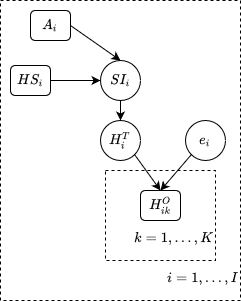
\includegraphics[width=\textwidth]{entropy_DAG2.png}
		\caption{}
	\end{subfigure}
	\hspace{0.1\textwidth}
	\begin{subfigure}{0.425\textwidth}
		\centering
		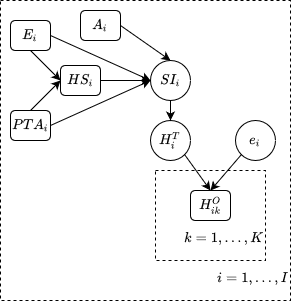
\includegraphics[width=\textwidth]{entropy_DAG1.png}
		\caption{}
	\end{subfigure}
	%
	\caption[DAG for the hierarchical beta regression model for entropy.]%
	{DAG for the hierarchical beta regression model for entropy. (a) \textit{total effects} of hearing status, (b) \textit{direct effects} of hearing apparatus. Circles represent latent variables, squares observed values or covariates, and large discontinuous squares the nesting within specific units.}
	\label{fig:entropy_ME}
\end{figure}
%

First, figure \ref{fig:entropy_ME} depicts the DAG representation of the model. For the measurement error part, section \ref{ss_sect:outcome} reveals the (observed) entropy replicates $H^{O}_{ik}$ can represent multiple realizations of a child's \textit{true} entropy $H^{T}_{i}$, measured with error $e_i$. As a result, we can say the $k$'th entropy measure is nested within the $i$'th child, where $k=1, \dots, K$, $i=1, \dots, I$, $K = 10$ utterances, and $I = 32$ children.

Second, for the hypothesis part, we can say the child's \textit{true} entropy $H^{T}_{i}$ is inversely explained by the child's speech intelligibility index $SI_{i}$, and in turn, the latter by a set of covariates. Notice from Figure \ref{fig:entropy_ME}, we propose two sets of models. The model in panel (a) use hearing status ($HS_{i}$) and hearing age ($A_{i}$) as covariates. The use of hearing status is justified as we are interested in comparing SI among groups, defined by the children's hearing characteristics (NH, HI/CI, and HI/HA). On the other hand, we expect hearing age\footnote{see section \ref{s_sect:children} to know how the variable is defined.} and its interaction with hearing status, to also have an effect on the SI index, as previous evidence have shown the speech of HI children gradually approximate that of NH children \citep{Boonen_et_al_2019}.

Notice the model depicted in panel (a) is interested on (what we can call) \textit{total effects}, i.e. the effects of the hearing characteristics, not independent from the effects of the hearing apparatus (cochlear implant or hearing aid). This is important to understand for two reasons. Since a hearing apparatus is fitted onto a child depending on aspects such as the locus and severity of his(her) hearing impairment \citep{Korver_et_al_2017}: (1) such specific children's characteristics could confound the (beneficial) effects of using specific hearing apparatuses, while (2) because children are selected from a convenient sample, not representative of their respective populations (see section \ref{s_sect:children}), the need to control for such characteristics is paramount, if we seek to obtain effects that can generalize better and beyond our sample\footnote{follow the \textit{notes} folder, to see a graphical though experiment.}.

Considering the previous, we propose the model depicted in panel (b), where we control for the possible confounding variables etiology ($E_{i}$), \textcolor{blue}{as a proxy of locus}, and unaided PTA ($PTA_{i}$), as a proxy for hearing impairment severity. In that sense, the model would estimate (what we can call) the \textit{direct effects} of the hearing apparatus, independent of the children's characteristics.

Lastly, we proceed to use probabilistic programming to declare the algebraic structure of our models. Given the panel (a) model is nested within the panel (b) model, we declare only the model structure for the latter:
%
\begin{align}
	%
	\text{Likelihood:} & \nonumber \\
	%
	H^{O}_{ik} & \sim \text{BetaProp} \left( H^{T}_{i}, M_{i} \right) \\ 
	%
	\nonumber \\
	%
	%
	\text{Transformed parameters:} & \nonumber \\
	%
	H^{T}_{i} &= \text{logit}^{-1}( -SI_{i} ) \\
	%
	\nonumber \\
	%
	%
	\text{Linear predictor:} & \nonumber \\
	SI_{i} & = a_{i} + \alpha + \alpha_{HS[i]} + \beta_{A, HS[i]} (A_{i} - \bar{A}) + \alpha_{E[i]} + \beta_{P} PTA_{i} \\ 
	%
	\nonumber \\
	%
	%
	\text{Priors:} & \nonumber \\
	%
	M_{i} & \sim \text{LN}( \mu_{M}, \sigma_{M}) \\
	%
	a_{i} & \sim \text{N}(\mu_{a}, \sigma_{a}) \\
	%
	\alpha & \sim \text{N}(0, 0.5) \\
	\alpha_{HS[i]} & \sim \text{N}(0, 0.5) \\
	%
	\beta_{A, HS[i]} & \sim \text{N}(0 , 0.3) \\
	%
	\alpha_{E[i]} & \sim \text{N}(0, 0.5) \\
	%
	\beta_{P} & \sim \text{N}(0, 0.3) \\
	%
	\nonumber \\
	%
	%
	\text{Hyper-priors:} & \nonumber \\
	%
	\mu_{M} & \sim \text{N}(0, 5) \\
	\sigma_{M} & \sim \text{Exp}(1) \\
	\mu_{a} & \sim \text{N}(0, 0.5) \\
	\sigma_{a} & \sim \text{Exp}(1)\\
	%
\end{align}
%
where $\text{logit}(x) = \log \left[ x / ( 1 - x ) \right]$, and $\text{logit}^{-1}(x) = \exp(x) / ( 1 + \exp(x) ) $. Additionally, a $\text{BetaProp}(\mu, \theta)$ distribution is equal to a $\text{Beta}(\alpha, \beta)$ distribution, with $\alpha=\mu \theta$, $\beta=(1-\mu)\theta$. For our purposes, $\mu = H^{T}_{i}$ and $\theta = M_{i}$, the latter denoting the ``sample size" of the distribution. Moreover, $a_{i}$ denote the children's random effects, $\alpha$ the fixed effects' intercept, $\alpha_{HS[i]}$ and $\beta_{A, HS[i]}$ the intercept and slope of ``hearing age" per hearing status group, $\alpha_{E[i]}$ the intercept per etiology group, and $\beta_{P}$ the slope for the standardized PTA levels. 

Four important things need to be noticed from the previous algebraic structure. First, all the parameters are estimated in the logit scale and centered at $PTA_{i}=0$ and $\bar{A}$, which denotes the minimum hearing age in the sample. Second, instead of a latent measurement error $e_i$, we use the latent ``sample size" parameter $M_{i}$ to model the heterogeneity/variability of the duplicate entropies. This effectively works as a measurement error model for the duplicates, as the parameter defines the shape of the distribution. Third, we use mildly informative priors to state our uncertainty regarding the direction and magnitude of the effects\footnote{see \citet{Rivera_2021} (p. 18-19) for an intuition on prior elicitation.}. Fourth, if we do not consider etiology and PTA values in equation (4), we obtain the panel (a) model.
%
%

\subsubsection{Priors}

\subsubsection{Estimation}
The models proposed in sections \ref{s_sect:evaluation} and \ref{s_sect:models} will be estimated under the Bayesian framework\footnote{see \citet{Rivera_2021} (p. 11-13, 15-27) for a detailed description of its benefits and shortcomings.}. More specifically, we will use the No-U-Turn Hamiltonian Monte Carlo algorithm (No-U-Turn HMC) \citep{Betancourt_et_al_2013, Duane_et_al_1987, Hoffman_et_al_2014, Neal_2012}. \texttt{Stan} \citep{Stan_2020} will be the software package that will provide us with the No-U-Turn HMC machinery, while \texttt{R} \citep{R_2015} and its integration packages \citep{RStan_2020}, the software that will allow us to analyze its outputs.


\subsubsection{Pre-processing} \label{ss_sect:preproc}
%
Besides the exclusion of corrupted observations, e.g. no available rating, no other experimental run nor duplicate was eliminated before the modeling process. This decision departs from what it is observed in previous research, e.g. \citet{Boonen_et_al_2020} decided to eliminate "outlying" observations based on misfit analysis \citep{Lesterhuis_2018}, while \citet{vanDaal_2020} and \citet{Boonen_et_al_2021} did the same based on univariate outlier analysis. 

For the case of misfit analysis, we argue that such procedures cannot be used without caution. The literature points out that in the context of CJ, these statistics are always relative, i.e. they depend on other stimulus and judges included in the assessment \citep{Pollitt_2012a, Pollitt_2012b}. Moreover, they have been proven to be less sensitive, as they are calculated with a low number of judgments per representation \citep{Pollitt_2012a}. 

On the other hand, for the case of univariate outlier analysis, we argue that outlying observations are interesting cases to analyze \citep{McElreath_2020}, and usually they cannot be identified properly outside the context of a full model \citep{McElreath_2020}, i.e. what can behave as an outlier based on a univariate analysis, can behave as expected under the appropriate model. 

Considering the previous, if we still manage to identify outlying observations within the context of the proposed models (see Section \ref{s_sect:models}), the researcher would rather make the model robust against their influence, playing on the strengths of the bayesian framework, than to eliminate the observations. 




%-------------------------------
\subsection{Simulation}
%-------------------------------
Preliminary to the data collection, we simulated data in silico to test the models and inform data collection procedure. The simulation code is available in the GitHub repository. Several functional correlation between age and knowledge have been simulated, and the model used in the analysis - which includes age as a ordinal categorical predictor of knowledge with monotonically increasing effect - has been able to recover the different shapes. Causal effect of activities, family composition and schooling have been simulated and tested.

The simulated data have been used -albeit in a previous version- to estimate the minimum number of interviewees necessary to recover the parameter values. If individuals were to name a maximum of 300 items in the freelist, 50 interviewees would have been suffcient to obtain reliable estimates of the parameters. Given that data collection in vivo is much less regular and less controllable than in silico, we roughly doubled the number of interviewees and that of questions.


%-------------------------------
\subsection{Model selection}
%-------------------------------
%
Following the successful and comprehensive analysis in \citet{vanDaal_2020} and \citet{Lesterhuis_2018}, the current research will also use the Information-Theoretic Approach (ITA) \citep{Anderson_2008, Chamberlain_1965} for the selection of competing models. The approach considers three steps: (1) state our hypothesis into statistical models, (2) select among competing models, and (3) make inferences based on one or multiple models.

First, for the translation of our working hypotheses into statistical models, we will use Directed Acyclic Graphs (DAG) and probabilistic programming \citep{Jaynes_2003}. A DAG is the simplest representation of a Graphical Causal Model (GCM), a heuristic model that contains information not purely statistical, but unlike a detailed statistical model, it allow us to deduce which variable relationships can provide valid causal inferences \citep{Hernan_et_al_2020, McElreath_2020}. In summary, a DAG is a reasonable way to state our hypothesis, and make our assumption more transparent. However, abide by the \textit{no-free lunch} rule, the causal inferences produced under the DAG will only be valid if the assumed DAG is correct. In contrast, the probabilistic programming will serve as the algebraic formalist to define our statistical models.

Second, to select among competing models, we will use the Widely Applicable Information Criterion (WAIC) \citep{Watanabe_2013}, and the Pareto-smoothed importance sampling cross-validation (PSIS) \citep{Vehtari_et_al_2021}\footnote{\citet{vanDaal_2020} used the Akaike’s Information Criterion (AIC) \citep{Akaike_1974} with similar purposes.}. Two reasons justify our decision. First, both criteria allow us to embrace the full flexibility and information of our bayesian implementation (outlined in Section \ref{s_sect:models}). Last, and more important, both criteria provide us with the best approximations for the out-of-sample (cross-validated) deviance \citep{McElreath_2020}. The deviance is the best approximation for the Kullback-Liebler (KL) divergence \citep{Kullback_et_al_1951}, i.e. a measure of how far a model is from describing the \textit{true} distribution of our data. \citet{McElreath_2020} points out that is a rather benign characteristic of the model's selection procedure that we do not need the KL divergence's absolute value, as the \textit{true} distribution of our data is not available (otherwise, we would not need a statistical model). But rather, using the difference in deviance between competing models, we can measure which model is the farthest from \textit{perfect (predictive) accuracy} for our data\footnote{see \citet{McElreath_2020} (p. 202-211) for the intuition and detailed derivation of the argument.}.

Finally, considering the evidence provided by the previous step, we proceed to make inferences based on one or multiple models.